\documentclass[tikz,border=2pt]{standalone}
\usepackage{amsmath}
\usepackage{pgfplots}
\pgfplotsset{compat=1.18}

\begin{document}
% Along a direction h from x_0 the function t -> f(x_0 + t h) is approximated by the tangent
% (first order, gradient) and by a parabola (second order, Hessian).
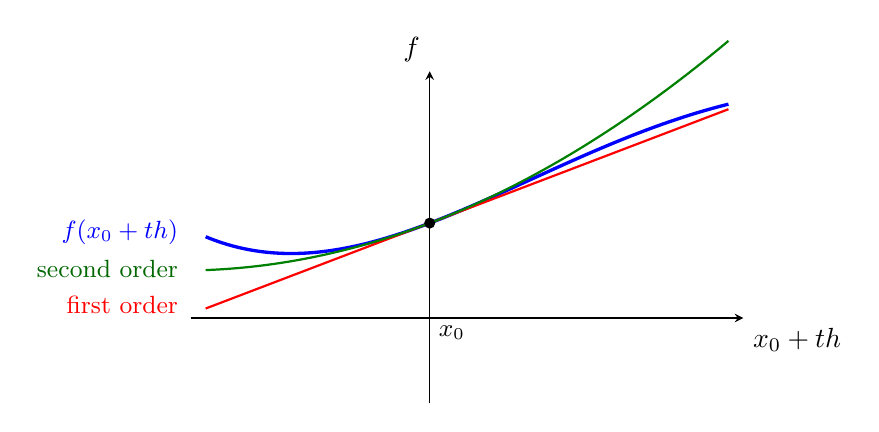
\begin{tikzpicture}
	\begin{axis}[
		axis lines=middle, xmin=-1.6, xmax=2.1, ymin=-0.9, ymax=2.6,
		xtick=\empty, ytick=\empty,
		xlabel={$x_0+th$}, ylabel={$f$}, xlabel style={below right}, ylabel style={above left},
		samples=120, smooth, width=8.6cm, height=5.8cm, clip=false
		]
		\addplot[blue, very thick, domain=-1.5:2.0] {exp(0.6*x)-0.4*x^3/3};
		\addplot[red, thick, domain=-1.5:2.0] {1+0.6*x};
		\addplot[green!50!black, thick, domain=-1.5:2.0] {1+0.6*x+0.18*x^2};
		\fill (axis cs:0,1) circle (2pt);
		\node[blue, anchor=east, font=\small] at (axis cs:-1.62,0.9) {$f(x_0+th)$};
		\node[green!40!black, anchor=east, font=\small] at (axis cs:-1.62,0.52) {second order};
		\node[red, anchor=east, font=\small] at (axis cs:-1.62,0.14) {first order};
		\node[anchor=north west, font=\small, inner sep=1.5pt] at (axis cs:0.03,-0.03) {$x_0$};
	\end{axis}
\end{tikzpicture}
\end{document}
